
\documentclass[border=8pt, multi, tikz]{standalone}
\usepackage{import}
\usepackage{graphicx}
\subimport{../layers/}{init}
\usetikzlibrary{positioning}
\usetikzlibrary{3d} %for including external image
\usetikzlibrary{decorations,shapes}
\usetikzlibrary{decorations.shapes}
\usetikzlibrary{decorations.markings}

\def\ConvColor{rgb:yellow,5;red,2.5;white,5}
\def\ConvReluColor{rgb:yellow,5;red,5;white,5}
\def\PoolColor{rgb:red,1;black,0.3}
\def\UpsampleColor{rgb:green,5; white,2}
\def\DetectColor{rgb:red,5; white,2}
\def\UnpoolColor{rgb:blue,2;green,1;black,0.3}
\def\FcColor{rgb:blue,5;red,2.5;white,5}
\def\FcReluColor{rgb:blue,5;red,5;white,4}
\def\SoftmaxColor{rgb:magenta,5;black,7}
\def\SumColor{rgb:green, 1}
\def\ShortcutColor{rgb: blue, 3; green, 1; white, 5}
\def\MultColor{rgb: magenta, 1}
\def\ConcColor{rgb:red, 5}
\def\input_image{../examples/input_image.jpg}
\def\output_image{../examples/output_image.png}

\newcommand*{\drawMBoxes}[3]{%
	\foreach \i in {0,1,...,#3} {
		\draw [fill=white] (#1,#2-\i) rectangle (#1+1,#2-\i+1) node[pos=.5] {\Large $ p_{\i}$};
	}%
	\draw [fill=white] ({#1},{#2-(#3+1)}) rectangle ({#1+1},{#2-(#3+1)+1}) node[pos=.5] {\Large $\vdots$};
	\draw [fill=white] ({#1},{#2-(#3+2)}) rectangle ({#1+1},{#2-(#3+2)+1}) node[pos=.5] {\Large $ p_{40} $};
}%

\newcommand{\copymidarrow}{\tikz \draw[-Stealth,line width=0.8mm,draw={rgb:blue,4;red,1;green,1;black,3}] (-0.3,0) -- ++ (0.3,0);}

\begin{document}
    \begin{tikzpicture}
        \tikzstyle{fillwhite} = [fill=white,inner sep=0pt, opacity=1]
        \tikzstyle{connection}=[ultra thick,every node/.style={sloped,allow upside down},draw=\edgecolor,opacity=0.7]
        \tikzstyle{fuseconnection}=[ultra thick,every node/.style={sloped,allow upside down},draw=orange, decorate,decoration={markings,
            mark connection node=my node,
            mark=at position .8 with
            {\node [draw, fill=orange, rectangle, minimum height = 4mm, minimum width=1mm,
            transform shape, inner sep=0pt] (my node) {};}}], opacity=0.7]

        %\tikzstyle{fuseconnection}=[ultra thick,every node/.style={sloped,allow upside down},draw=orange, decorate,decoration={shape backgrounds,shape=signal, shape size=.2mm, shape sep={2mm, between borders}}, signal from=west, signal pointer angle = 5]
        %\tikzstyle{fuseconnection}=[ultra thick,every node/.style={sloped,allow upside down},draw=orange]
        \tikzstyle{copyconnection}=[ultra thick,every node/.style={sloped,allow upside down},draw={rgb:blue,4;red,1;green,1;black,3},opacity=0.7]

        \node[canvas is zy plane at x=1] (image_0) at (-4,0,0) {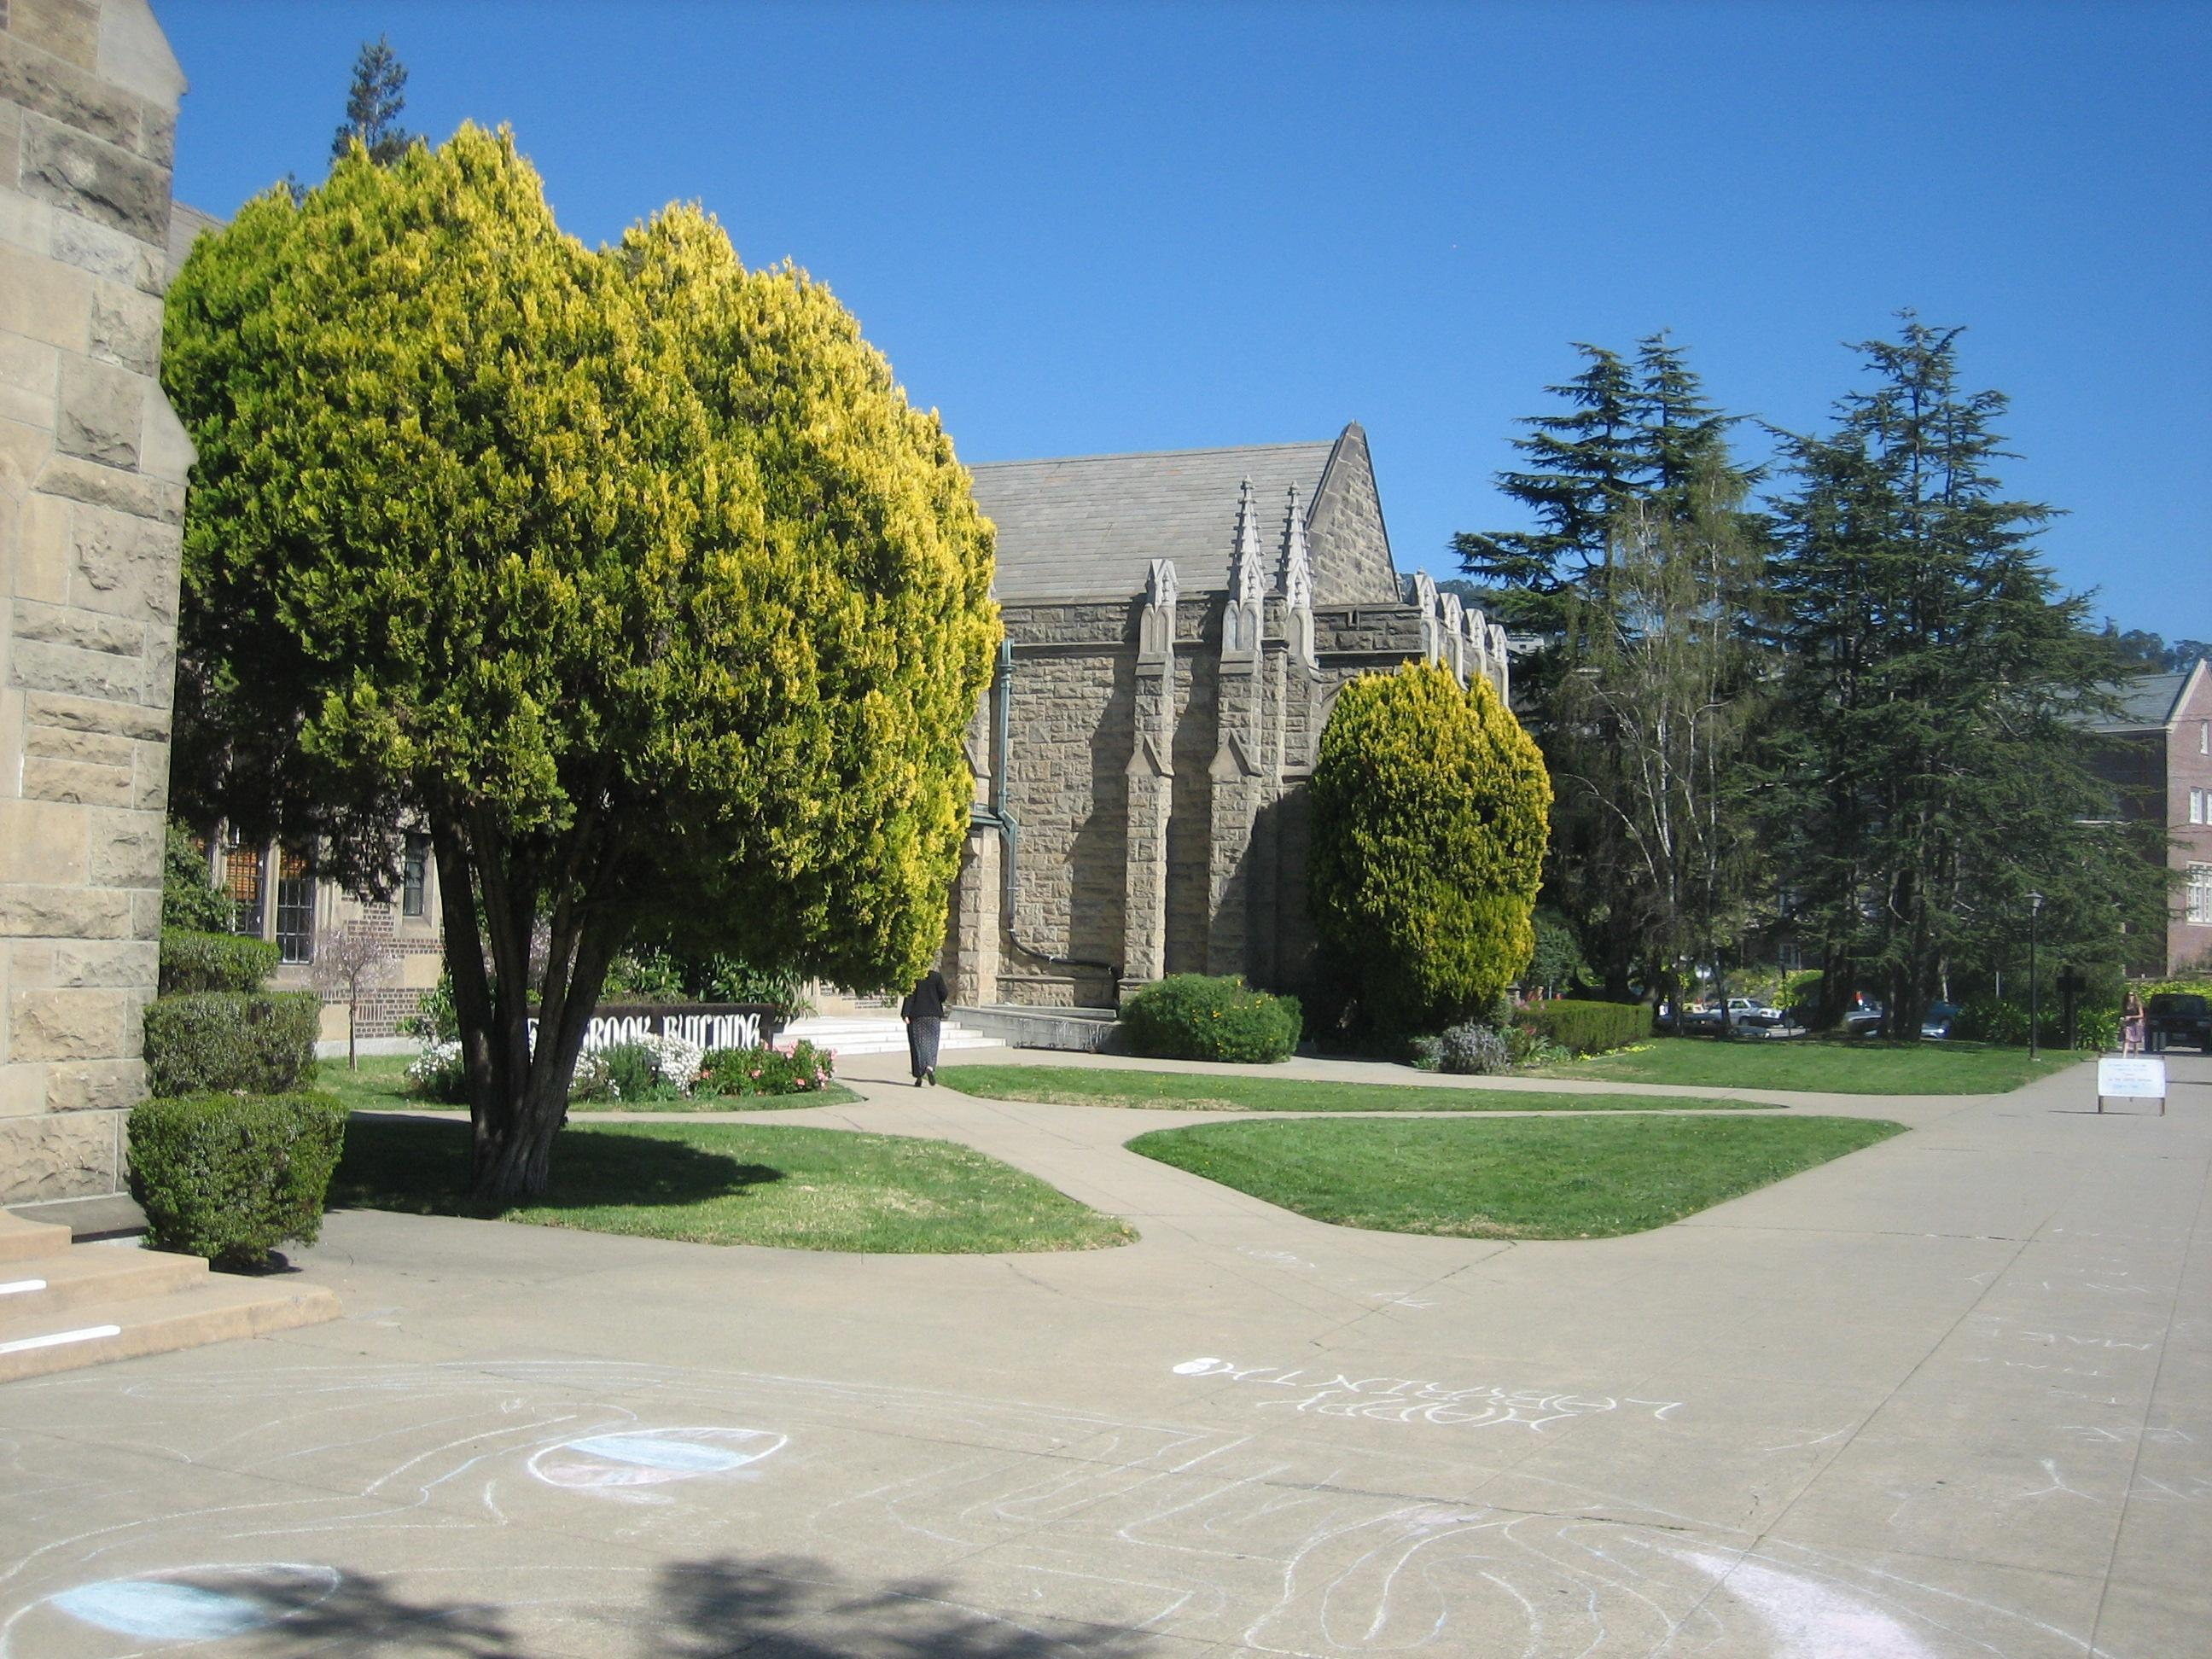
\includegraphics[width=10cm ,height=10cm ]{\input_image}};

        \pic[shift={(1, 0, 0)}, ] at (0,0,0)
            {RightBandedBox={
                name=conv_1,
                caption=,
                xlabel={(3,)},
                zlabel=I,
                fill=\ConvColor,
                bandfill=\ConvReluColor,
                height=32,
                depth=32,
                width={0.7924812503605781}
                }
            };

        \pic[shift={(3, 0, 0)}] at (conv_1-east)
            {Box={
                name=pool_1,
                caption= ,
                fill=\PoolColor,
                opacity=0.5,
                height=32,
                depth=32,
                width=1,
                }
            };

  \pic[shift={(2, 0, 0)}, ] at (pool_1-east)
{RightBandedBox={
		name=conv_2,
		caption=,
		xlabel={(96,)},
		zlabel=I/2,
		fill=\ConvColor,
		bandfill=\ConvReluColor,
		height=16.0,
		depth=16.0,
		width={3.292481250360578}
	}
};


        \draw [connection, ] (conv_1-east) -- node  {\midarrow}(pool_1-west);


        \draw[densely dashed]
            (pool_1-nearnortheast) coordinate(a) -- (conv_2-nearnorthwest)
            (pool_1-nearsoutheast) coordinate(b) -- (conv_2-nearsouthwest)
            (pool_1-farsoutheast) coordinate(c) -- (conv_2-farsouthwest)
            (pool_1-farnortheast) coordinate(d) -- (conv_2-farnorthwest)
            ;
    
        \draw [connection, ] (pool_1-east) -- node  {\midarrow}(conv_2-west);

        \pic[shift={(2, 0, 0)}] at (conv_2-east)
            {Box={
                name=pool_2,
                caption= ,
                fill=\PoolColor,
                opacity=0.5,
                height=16.0,
                depth=16.0,
                width=1,
                }
            };

        \draw [connection, ] (conv_2-east) -- node  {\midarrow}(pool_2-west);

        \pic[shift={(2, 0, 0)}, ] at (pool_2-east)
            {RightBandedBox={
                name=conv_4_6_0,
                caption=,
                xlabel={(384,)},
                zlabel=,
                fill=\ConvColor,
                bandfill=\ConvReluColor,
                height=8.0,
                depth=8.0,
                width={4.292481250360578}
                }
            };

        \pic[shift={(0,0,0)}, ] at (conv_4_6_0-east)
            {RightBandedBox={
                name=conv_4_6_1,
                caption=,
                xlabel={(384,)},
                zlabel=,
                fill=\ConvColor,
                bandfill=\ConvReluColor,
                height=8.0,
                depth=8.0,
                width={4.292481250360578}
                }
            };

        \pic[shift={(0,0,0)}, ] at (conv_4_6_1-east)
            {RightBandedBox={
                name=conv_4_6_2,
                caption=,
                xlabel={(256,)},
                zlabel=I/4,
                fill=\ConvColor,
                bandfill=\ConvReluColor,
                height=8.0,
                depth=8.0,
                width={4.0}
                }
            };

        \draw [connection, ] (pool_2-east) -- node  {\midarrow}(conv_4_6_0-west);

        \draw[densely dashed]
            (pool_2-nearnortheast) coordinate(a) -- (conv_4_6_0-nearnorthwest)
            (pool_2-nearsoutheast) coordinate(b) -- (conv_4_6_0-nearsouthwest)
            (pool_2-farsoutheast) coordinate(c) -- (conv_4_6_0-farsouthwest)
            (pool_2-farnortheast) coordinate(d) -- (conv_4_6_0-farnorthwest)
            ;
    
        \pic[shift={(1, 0, 0)}] at (conv_4_6_2-east)
            {Box={
                name=pool_3,
                caption= ,
                fill=\PoolColor,
                opacity=0.5,
                height=8.0,
                depth=8.0,
                width=1,
                }
            };

        \draw [connection, ] (conv_4_6_2-east) -- node  {\midarrow}(pool_3-west);

        \pic[shift={(1, 0)}] at (pool_3-east)
            {Box={
                name=fully_1,
                caption= ,
                xlabel={(4096,)},
                zlabel=,
                fill=\UpsampleColor,
                height=4.0,
                width=8.317766166719343,
                depth={4.0}
                }
            };

        \draw [connection, ] (pool_3-east) -- node  {\midarrow}(fully_1-west);

        \draw[densely dashed]
            (pool_3-nearnortheast) coordinate(a) -- (fully_1-nearnorthwest)
            (pool_3-nearsoutheast) coordinate(b) -- (fully_1-nearsouthwest)
            (pool_3-farsoutheast) coordinate(c) -- (fully_1-farsouthwest)
            (pool_3-farnortheast) coordinate(d) -- (fully_1-farnorthwest)
            ;
    
        \pic[shift={(1, 0)}] at (fully_1-east)
            {Box={
                name=fully_2,
                caption= ,
                xlabel={(4096,)},
                zlabel=,
                fill=\UpsampleColor,
                height=4.0,
                width=8.317766166719343,
                depth={4.0}
                }
            };

        \draw[densely dashed]
            (fully_1-nearnortheast) -- (fully_2-farnorthwest)
            (fully_1-nearnortheast) -- (fully_2-nearnorthwest)
            (fully_1-farnortheast) -- (fully_2-nearnorthwest)
            (fully_1-farnortheast) -- (fully_2-farnorthwest)
            (fully_1-farnortheast) -- (fully_2-nearsouthwest)
            (fully_1-nearsoutheast) -- (fully_2-farsouthwest)
            (fully_1-nearsoutheast) -- (fully_2-nearsouthwest)
            (fully_1-nearsoutheast) -- (fully_2-farnorthwest)
            (fully_1-farsoutheast) --(fully_2-nearsouthwest)
            (fully_1-farsoutheast) --(fully_2-farsouthwest);

        \pic[shift={(1, 0)}] at (fully_2-east)
            {Box={
                name=fully_3,
                caption= ,
                xlabel={(40,)},
                zlabel=,
                fill=\UpsampleColor,
                height=4.0,
                width=3.6888794541139363,
                depth={4.0}
                }
            };

        \draw[densely dashed]
            (fully_2-nearnortheast) -- (fully_3-farnorthwest)
            (fully_2-nearnortheast) -- (fully_3-nearnorthwest)
            (fully_2-farnortheast) -- (fully_3-nearnorthwest)
            (fully_2-farnortheast) -- (fully_3-farnorthwest)
            (fully_2-farnortheast) -- (fully_3-nearsouthwest)
            (fully_2-nearsoutheast) -- (fully_3-farsouthwest)
            (fully_2-nearsoutheast) -- (fully_3-nearsouthwest)
            (fully_2-nearsoutheast) -- (fully_3-farnorthwest)
            (fully_2-farsoutheast) --(fully_3-nearsouthwest)
            (fully_2-farsoutheast) --(fully_3-farsouthwest);

        \pic[shift={(2, 0, 0)}] at (fully_3-west)
            {Box={
                name=soft_max,
                caption= ,
                xlabel={{40,}},
                zlabel=,
                fill=\SoftmaxColor,
                opacity=0.8,
                height=4.0,
                depth=4.0,
                width=1.5
                }
            };

        \draw [connection, ] (fully_3-east) -- node  {\midarrow}(soft_max-west);
        
    	\drawMBoxes{25}{2.5}{4}	
        
        \draw [connection, ] (soft_max-east) -- node  {\midarrow}(25,0);
        
        \end{tikzpicture}
        \end{document}
    